\documentclass{article}
\usepackage[utf8]{inputenc}
\usepackage[margin=1in]{geometry}
\usepackage{soul,color}
\usepackage{amsfonts, amsmath}
\usepackage{bbm}
\usepackage{enumitem}
\usepackage[nobreak=true]{mdframed}
\usepackage{amssymb}
\usepackage{graphicx}

\newcommand{\solution}{\textbf{Solution: }}
\newcommand{\N}{\mathcal{N}}
% \newcommand{\Pbf}{\textbf{P}}
\newcommand{\R}{\mathbb{R}}
\newcommand{\E}{\mathbb{E}}
\newcommand{\Var}{\text{Var}}
\newcommand{\Cov}{\text{Cov}}
\newcommand{\Ell}{\mathcal{L}}

\usepackage[utf8]{inputenc}

% Default fixed font does not support bold face
\DeclareFixedFont{\ttb}{T1}{txtt}{bx}{n}{8} % for bold
\DeclareFixedFont{\ttm}{T1}{txtt}{m}{n}{8}  % for normal

% Custom colors
\usepackage{color}
\definecolor{deepblue}{rgb}{0,0,0.5}
\definecolor{deepred}{rgb}{0.6,0,0}
\definecolor{deepgreen}{rgb}{0,0.5,0}

\usepackage{listings}

% Python style for highlighting
\newcommand\pythonstyle{\lstset{
language=Python,
basicstyle=\ttfamily\footnotesize,
otherkeywords={self},             % Add keywords here
keywordstyle=\ttb\color{deepblue},
emph={MyClass,__init__},          % Custom highlighting
emphstyle=\ttb\color{deepred},    % Custom highlighting style
stringstyle=\color{deepgreen},
frame=tb,                         % Any extra options here
showstringspaces=false           % 
}}


% Python environment
\lstnewenvironment{python}[1][]
{
\pythonstyle
\lstset{#1}
}
{}

% Python for external files
\newcommand\pythonexternal[2][]{{
\pythonstyle
\lstinputlisting[#1]{#2}}}

% Python for inline
\newcommand\pythoninline[1]{{\pythonstyle\lstinline!#1!}}

\title{CS189, HW3: Gaussians}
\author{ Completed by: Matthew Wu}
% \date{January 2017}
\date{}

\begin{document}

\maketitle

\subsection*{1. Independence vs. Correlation}
\begin{enumerate}[label=(\alph*)]
    \item Consider the random variables $X, Y \in \R$ with the following conditions.
    \begin{enumerate}[label=(\roman*)]
        \item $X$ and $Y$ can take values $\{-1, 0, 1\}$. 
        \item Either $X$ is 0 with probability $(\frac{1}{2})$, or $Y$ is 0 with probability $(\frac{1}{2})$.
        \item When $X$ is 0, $Y$ takes values 1 and -1 with equal probability $(\frac{1}{2})$. When $Y$ is 0, $X$ takes values 1 and -1 with equal probability $(\frac{1}{2})$.
    \end{enumerate}
    
    Are $X$ and $Y$ uncorrelated? Are $X$ and $Y$ independent. Prove your assertions. \emph{Hint:} Graph these points in the plane. What’s each point’s joint probability?
    
    \begin{mdframed} \solution\\
    $P(X=0,Y=1)=P(X=0,Y=-1)=P(X=1,Y=0)=P(X=-1,Y=0)=\frac{1}{4}$\\
    $P(X=0)=P(Y=0)=\frac{1}{2}$\\
    $P(X=0 \wedge Y=0)=0 \neq \frac{1}{4} = P(X=0)*P(Y=0)$, so $X$ and $Y$ are dependent.
    \end{mdframed}
    
    \item Consider three Bernoulli random variables $B, C,$ and $D$ which take values $\{0, 1\}$ with equal probability. Construct three more random variables $X, Y, Z$ such that $X = B \oplus C, Y = C \oplus D$, and $Z = B \oplus D$, where $\oplus$ is the XOR (exclusive or) operator. Are $X, Y,$ and $Z$ pairwise independent? Mutually independent? Prove it.
    
    \begin{mdframed} \solution All of the following outcomes have equal probability.
    \[
    \begin{tabular}{|c|c|c|c|}
    \hline
    B & C & D & (X, Y, Z)\\\hline
    0 & 0 & 0 & (0, 0, 0)\\\hline
    0 & 0 & 1 & (0, 1, 1)\\\hline
    0 & 1 & 0 & (1, 1, 0)\\\hline
    0 & 1 & 1 & (1, 0, 1)\\\hline
    1 & 0 & 0 & (1, 0, 1)\\\hline
    1 & 0 & 1 & (1, 1, 0)\\\hline
    1 & 1 & 0 & (0, 1, 1)\\\hline
    1 & 1 & 1 & (0, 0, 0)\\\hline
    \end{tabular}
    \]
    $P(X=0)=P(Y=0)=P(Z=0)=P(X=1)=P(Y=1)=P(Z=1)\frac{1}{2}$\\
    $P(X=x \wedge Y=y)=P(X=x)P(Y=y)=\frac{1}{4}\quad \forall x, y \in \{0, 1\}$\\
    $P(X=x \wedge Z=z)=P(X=x)P(Z=z)=\frac{1}{4}\quad \forall x, z \in \{0, 1\}$\\
    $P(Y=y \wedge Z=z)=P(Y=y)P(Z=z)=\frac{1}{4}\quad \forall y, z \in \{0, 1\}$\\
    $\therefore$ $X,Y,Z$ are pairwise independent.\\
    $P(X=1 \wedge Y=0 \wedge Z=0)=0 \neq \frac{1}{8}=P(X=1)P(Y=0)P(Z=0)$\\
    $\therefore$ $X,Y,Z$ are not mutually independent.
    \end{mdframed}
\end{enumerate}

\newpage
\subsection*{2. Isocontours of Normal Distributions}
Let $f(\mu, \Sigma)$ be the density function of a normally distributed random variable in $\R^2$. Plot isocontours of the following functions.
\begin{enumerate}[label=(\alph*)]
    \item $f(\mu, \Sigma)$, where $\mu = \begin{bmatrix}1 \\ 1 \end{bmatrix}$ and $\Sigma = \begin{bmatrix} 1 & 0  \\ 0 & 2 \end{bmatrix}$. 
    \begin{mdframed} \solution\\
    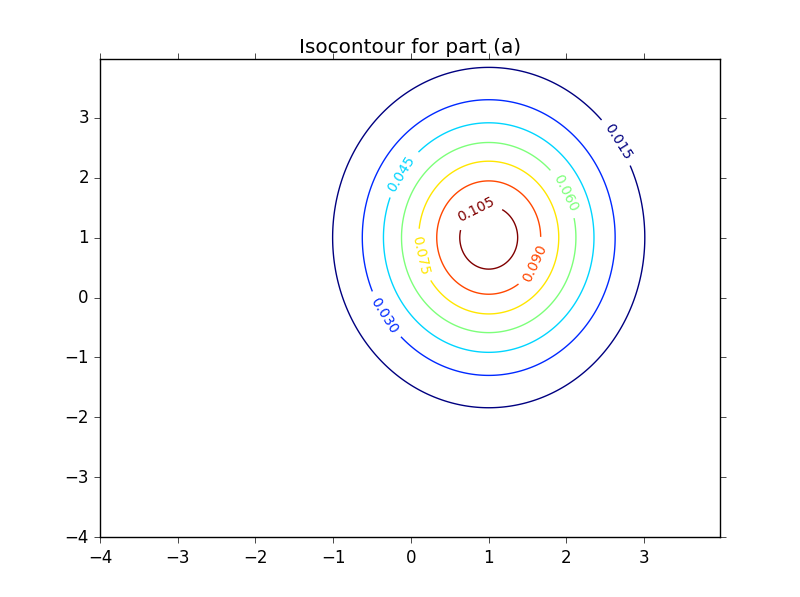
\includegraphics[scale=.75]{images/isocontour_a.png}
    \end{mdframed}
    
    \newpage
    \item $f(\mu, \Sigma)$, where $\mu = \begin{bmatrix}-1 \\ 2 \end{bmatrix}$ and $\Sigma = \begin{bmatrix} 2 & 1  \\ 1 & 3 \end{bmatrix}$. 
    \begin{mdframed} \solution\\
    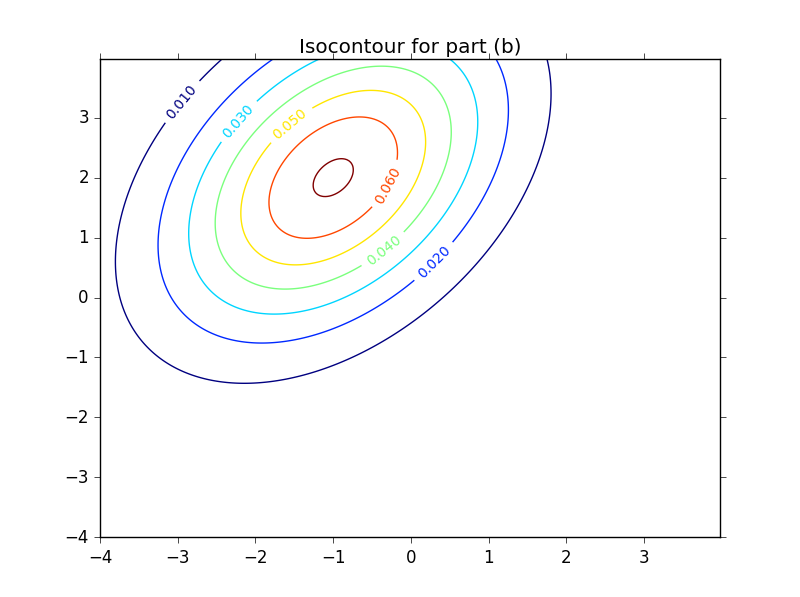
\includegraphics[scale=.75]{images/isocontour_b.png}
    \end{mdframed}
    
    \newpage
    \item $f(\mu_1, \Sigma_1) - f(\mu_2, \Sigma_2)$, where $\mu_1 = \begin{bmatrix} 0 \\ 2 \end{bmatrix}, \mu_2 = \begin{bmatrix} 2 \\ 0 \end{bmatrix}$ and $\Sigma_1 = \Sigma_2 = \begin{bmatrix} 2 & 1 \\ 1 & 1 \end{bmatrix}$. 
    \begin{mdframed} \solution\\
    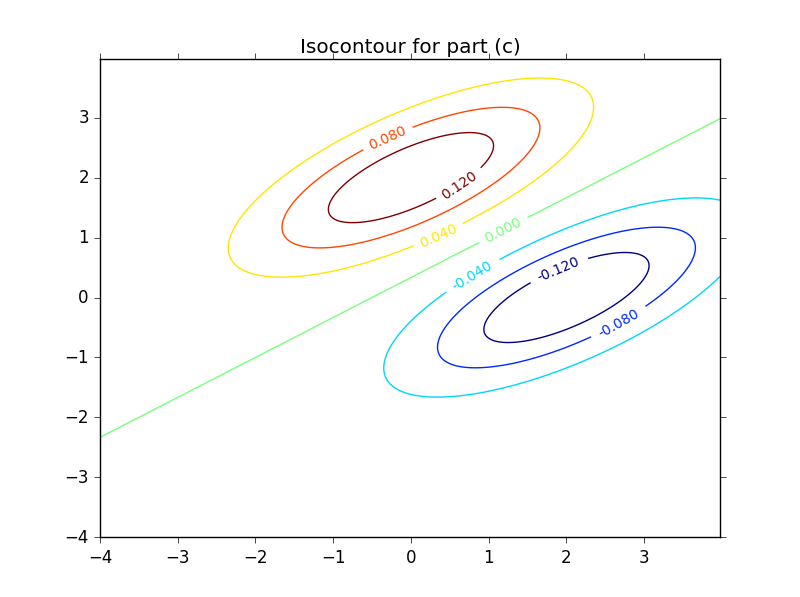
\includegraphics[scale=.75]{images/isocontour_c.png}
    \end{mdframed}
    
    \newpage
    \item $f(\mu_1, \Sigma_1) - f(\mu_2, \Sigma_2)$, where $\mu_1 = \begin{bmatrix} 0 \\ 2 \end{bmatrix}, \mu_2 = \begin{bmatrix} 2 \\ 0 \end{bmatrix}, \Sigma_1 = \begin{bmatrix} 2 & 1 \\ 1 & 1 \end{bmatrix}$ and $\Sigma_2 = \begin{bmatrix} 2 & 1 \\ 1 & 3 \end{bmatrix}$.
    \begin{mdframed} \solution\\
    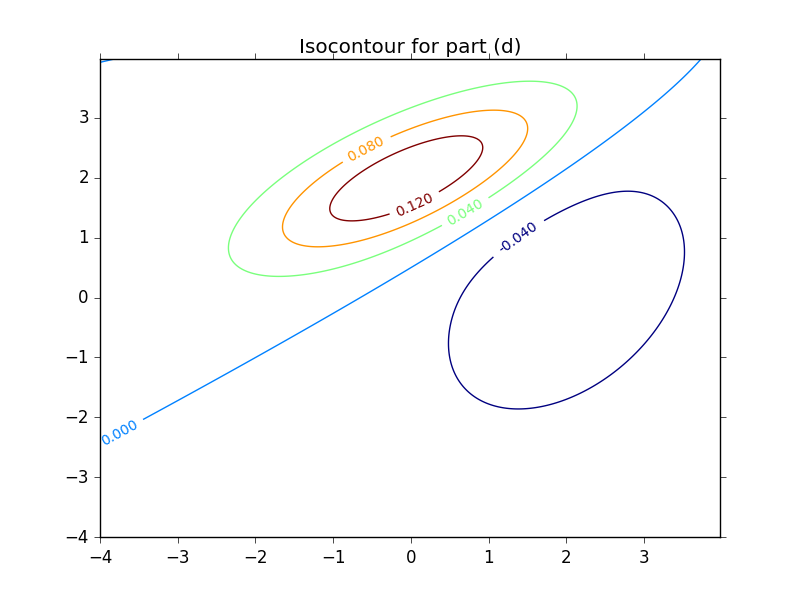
\includegraphics[scale=.75]{images/isocontour_d.png}
    \end{mdframed}
    
    \newpage
    \item $f(\mu_1, \Sigma_1) - f(\mu_2, \Sigma_2)$, where $\mu_1 = \begin{bmatrix} 1 \\ 1 \end{bmatrix}, \mu_2 = \begin{bmatrix} -1 \\ -1 \end{bmatrix}, \Sigma_1 = \begin{bmatrix} 2 & 0 \\ 0 & 1 \end{bmatrix}$ and $\Sigma_2 = \begin{bmatrix} 2 & 1 \\ 1 & 2 \end{bmatrix}$.
    \begin{mdframed} \solution\\
    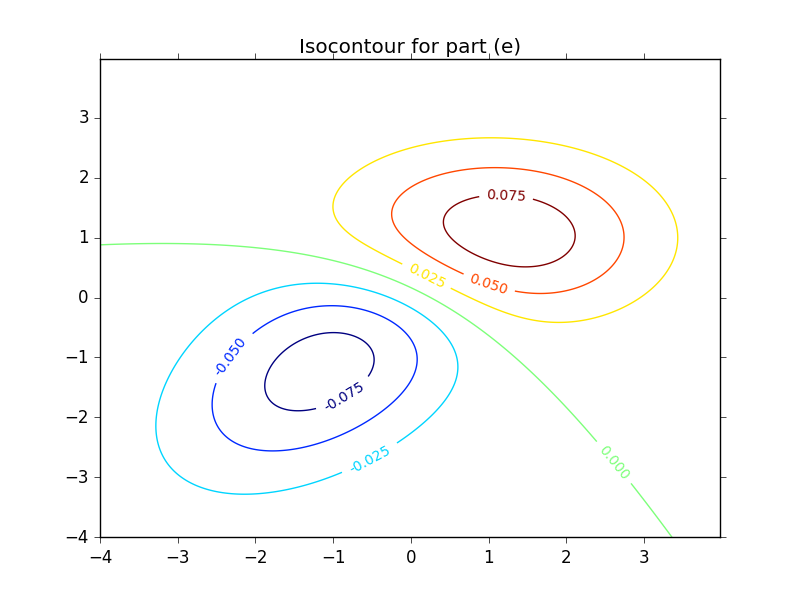
\includegraphics[scale=.75]{images/isocontour_e.png}
    \end{mdframed}
    
\end{enumerate}

\newpage
\subsection*{3. Eigenvectors of the Gaussian Covariance Matrix}
Consider two one-dimensional random variables $X_1 \sim \N(3, 9)$ and $X_2 \sim \frac{1}{2}X_1 + \N(4, 4)$, where $\N(\mu, \sigma^2)$  is a Gaussian distribution with mean $\mu$ and variance $\sigma^2$. In software, draw $N = 100$ random two-dimensional sample points from $(X_1, X_2)$ such that the $i$th value sampled from $X_2$ is calculated based on the $i$th value sampled from $X_1$. 
\begin{enumerate}[label=(\alph*)]
    \item Compute the mean (in $\R^2$) of the sample. 
    \begin{mdframed} \solution
    See appendix for code. The mean for the sample was $\approx$ (2.920, 5.640)
    \end{mdframed}
    
    \item Compute the $2 \times 2$ covariance matrix of the sample.
    \begin{mdframed} \solution
    See appendix for code. The covariance matrix of the sample was
    $$\approx\begin{bmatrix}
    8.315 & 3.350\\
    3.350 & 4.617\end{bmatrix}$$    
    \end{mdframed}
    
    \item Compute the eigenvectors and eigenvalues of this covariance matrix. 
    \begin{mdframed} \solution
    See appendix for code. The eigenvectors and eigenvalues for the matrix were:
    $$v_1\approx\begin{bmatrix}0.861\\0.508\end{bmatrix},\; \lambda_1\approx 10.292 \qquad v_2\approx\begin{bmatrix}-0.508\\0.861\end{bmatrix},\;\lambda_2\approx 2.639$$
    \end{mdframed}
    
    \item On a two-dimensional grid with a horizontal axis for $X_1$ with range $[-15, 15]$ and a vertical axis for $X_2$ with range $[-15, 15]$, plot
    \begin{enumerate}[label=(\roman*)]
        \item all $N=100$ data points, and
        \item arrows representing both covariance eigenvectors. The eigenvector arrows should originate at the mean and have magnitudes equal to their corresponding eigenvalues.
    \end{enumerate}
    \begin{mdframed} \solution
    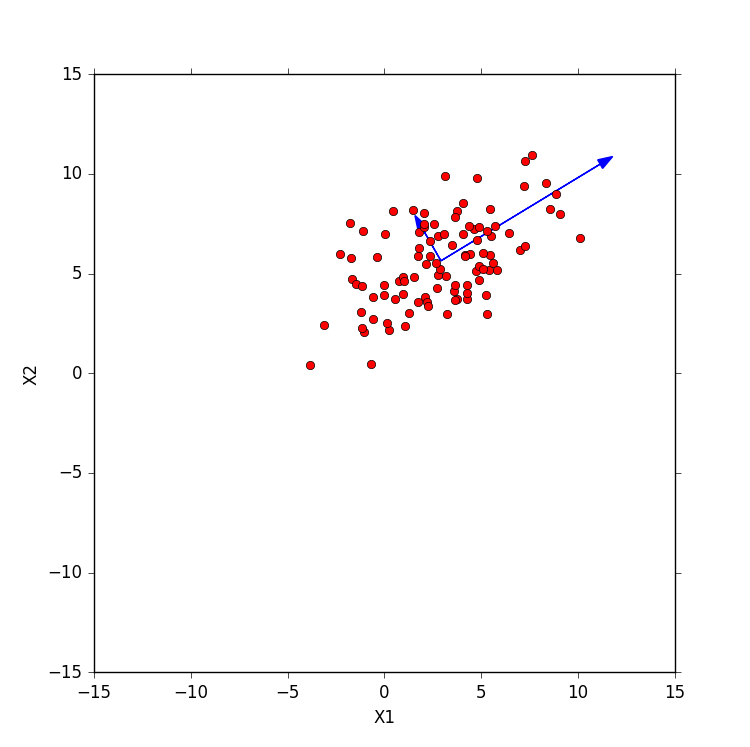
\includegraphics[scale=.5]{images/eigenvector_d.png}
    \end{mdframed}
    
    \item Let $U = \begin{bmatrix} v_1 & v_2 \end{bmatrix}$ be a $2 \times 2$ matrix whose columns are the eigenvectors of the covariance matrix, where $v_1$ is the eigenvector with the larger eigenvalue. We use $U^{\top}$ as a rotation matrix to rotate each sample point from the $(X_1, X_2)$  coordinate system to a coordinate system aligned with the eigenvectors. (As $U^{\top} = U^{-1}$, the matrix $U$ reverses this rotation, moving back from the eigenvector coordinate system to the original coordinate system). Center your sample points by subtracting the mean $\mu$ from each point; then rotate each point by $U^{\top}$, giving $x_{\text{rotated}} = U^{\top}(x - \mu)$.  Plot these rotated points on a new two dimensional-grid, again with both axes having range $[-15, 15]$. 
    \begin{mdframed} \solution
    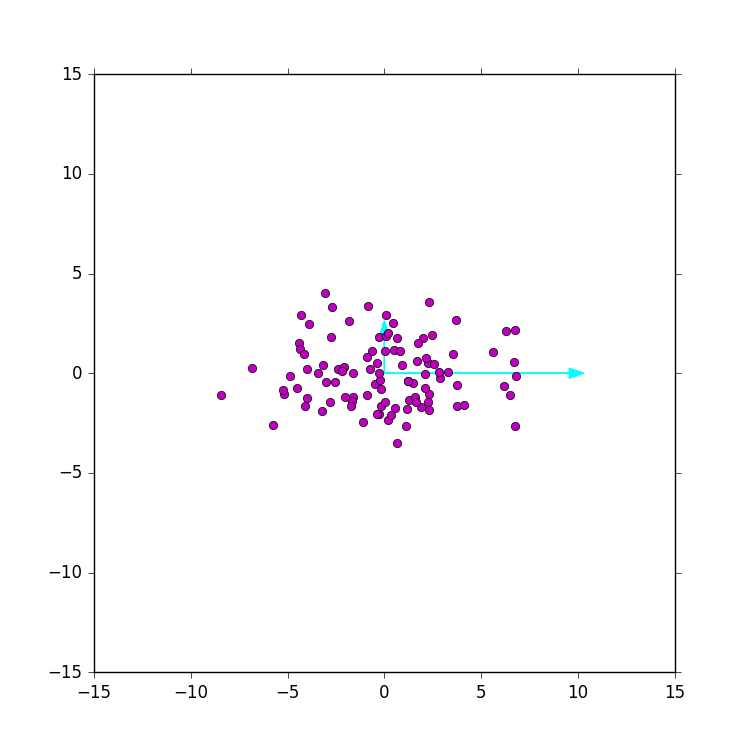
\includegraphics[scale=.5]{images/eigenvector_e.png}
    \end{mdframed}
    
\end{enumerate}

\newpage
\subsection*{4. Maximum Likelihood Estimation}
Let $X_1, \ldots, X_n \in \R^d$ be $n$ sample points drawn independently from a multivariate normal distribution $\N(\mu, \Sigma)$. 
\begin{enumerate}[label=(\alph*)]
    \item Suppose the normal distribution has an unknown diagonal covariance matrix
    $$
    \Sigma = 
    \begin{bmatrix}
    \sigma_1^2 & & & & \\
    & \sigma_2^2 & & & \\
    & & \sigma_3^2 & & \\
    & & & \ddots & \\
    & & & & \sigma_d^2 \\
    \end{bmatrix}
    $$
    and an unknown mean $\mu$. Derive the maximum likelihood estimates, denoted $\hat{\mu}$ and $\hat{\sigma_i}$ for $\mu$ and $\sigma_i$. Show all your work. 
    \begin{mdframed} \solution
    Suppose we have a normal distribution $X \sim N(\mu, \Sigma)$. Then we have:
    $$P(X_i)=\frac{1}{(\sqrt{2\pi})^d\sqrt{|\Sigma|}}\exp(-\frac{1}{2}(X_i-\mu)^T\Sigma^{-1}(X_i-\mu))\Rightarrow$$
    $$\Ell (\hat{\mu}, \hat{\Sigma})=\prod_{i=1}^n\frac{1}{(\sqrt{2\pi})^d\sqrt{|\hat{\Sigma}|}}\exp(-\frac{1}{2}(X_i-\hat{\mu})^T\hat{\Sigma}^{-1}(X_i-\hat{\mu}))$$
    $$=\frac{1}{(\sqrt{2\pi})^{nd}(\sqrt{|\hat{\Sigma}|})^n}\prod_{i=1}^n\exp(-\frac{1}{2}(X_i-\hat{\mu})^T\hat{\Sigma}^{-1}(X_i-\hat{\mu}))$$
    $$\ell=-\frac{nd}{2}\ln(2\pi)-\frac{n}{2}\ln(|\hat{\Sigma}|)-\frac{1}{2}\sum_{i=1}^n(X_i-\hat{\mu})^T\hat{\Sigma}^{-1}(X_i-\hat{\mu})$$
    $$\frac{\partial \ell}{\partial \hat{\mu}}=\sum_{i=1}^n\hat{\Sigma}^{-1}(X_i-\hat{\mu})=\hat{\Sigma}^{-1}\sum_{i=1}^n X_i-\hat{\mu}=0$$
    \center{Since $\hat{\Sigma}^{-1}$ is invertible, clearly}
    $$\sum_{i=1}^n X_i-\hat{\mu}=0\Rightarrow n\hat{\mu} = \sum_{i=1}^nX_i \Rightarrow \hat{\mu}=\frac{1}{n}\sum_{i=1}^n X_i$$
    Going back to our original equation for $\ell$, we can see
    $$\ell=-\frac{nd}{2}\ln(2\pi)-\frac{n}{2}\ln(\prod_{i=1}^{n}\hat{\sigma_i}^2)-\frac{1}{2}\sum_{i=1}^n\sum_{k=1}^n\frac{X_{ki}^2}{\hat{\sigma_i}^2}=-\frac{nd}{2}\ln(2\pi)-n\sum_{i=1}^n\ln(\hat{\sigma_i})-\frac{1}{2}\sum_{i=1}^n\frac{\sum_{k=1}^nX_{ki}^2}{\hat{\sigma_i}^2}$$
    $$\frac{\partial \ell}{\partial \hat{\sigma_i}}=-\frac{n}{\hat{\sigma_i}}+\frac{\sum_{k=1}^nX_{ki}^2}{\hat{\sigma_i}^3}\Rightarrow n\hat{\sigma_i}^2=\sum_{k=1}^nX_{ki}^2 \Rightarrow \hat{\sigma_i}=\sqrt{\frac{\sum_{k=1}^nX_{ki}^2}{n}}$$
    \end{mdframed}
    \newpage
    \item Suppose the normal distribution has a known covariance matrix $\Sigma$ and an unknown mean $A \mu$, where $\Sigma$ and $A$ are known $d \times d$ matrices, $\Sigma$ is positive definite, and $A$ is invertible.  Derive the maximum likelihood estimate, denoted $\hat{\mu}$, for $\mu$. \begin{mdframed} \solution
    We have a normal distribution $X \sim N(A\mu, \Sigma)$. This gives us:
    $$P(X_i)=\frac{1}{(\sqrt{2\pi})^d\sqrt{|\Sigma|}}\exp(-\frac{1}{2}(X_i-A\mu)^T\Sigma^{-1}(X_i-A\mu))\Rightarrow$$
    $$\Ell (\hat{\mu})=\prod_{i=1}^n\frac{1}{(\sqrt{2\pi})^d\sqrt{|\Sigma|}}\exp(-\frac{1}{2}(X_i-A\hat{\mu})^T\Sigma^{-1}(X_i-A\hat{\mu}))$$
    $$=\frac{1}{(\sqrt{2\pi})^{nd}(\sqrt{|\Sigma|})^n}\prod_{i=1}^n\exp(-\frac{1}{2}(X_i-A\hat{\mu})^T\Sigma^{-1}(X_i-A\hat{\mu}))$$
    $$\ell=-\frac{nd}{2}\ln(2\pi)-\frac{n}{2}\ln(|\Sigma|)-\frac{1}{2}\sum_{i=1}^n(X_i-A\hat{\mu})^T\Sigma^{-1}(X_i-A\hat{\mu})$$
    $$=C -\frac{1}{2}(\sum_{i=1}^nX_i^T\Sigma^{-1}X_i-2\sum_{i=1}^nX_i^T\Sigma^{-1}A\hat{\mu}+\sum_{i=1}^n\hat{\mu}^TA^T\Sigma^{-1}A\hat{\mu}) \text{ (since }(\Sigma^{-1})^T=\Sigma^{-1})$$
    $$\frac{\partial \ell}{\partial \hat{\mu}}=\sum_{i=1}^n(A^T\Sigma^{-1}X_i)-\sum_{i=1}^n(A^T\Sigma^{-1}A\hat{\mu})=0\Rightarrow$$
    $$n(A^T\Sigma^{-1}A\hat{\mu})=A^T\Sigma^{-1}\sum_{i=1}^nX_i$$
    $$n\hat{\mu}=A^{-1}\sum_{i=1}^nX_i$$
    $$\hat{\mu}=\frac{1}{n}A^{-1}\sum_{i=1}^nX_i$$
    \end{mdframed}
    
\end{enumerate}

\newpage
\subsection*{5. Covariance Matrices and Decompositions}
As described in lecture, the covariance matrix $\text{Var}(R) \in \R^{d\times d}$ for a random variable $R \in \R^d$ with mean $\mu$ is 
$$
\text{Var}(R) = \text{Cov}(R, R) = \E[(R- \mu)(R-\mu)^{\top}] = 
\begin{bmatrix}
\Var(R_1) & \Cov(R_1, R_2) & \ldots & \Cov(R_1, R_d) \\
\Cov(R_2, R_1) & \Var(R_2) & & \Cov(R_2, R_d) \\
\vdots & & \ddots & \vdots \\
\Cov(R_d, R_1) & \Cov(R_d, R_2) & \ldots & \Var(R_d)
\end{bmatrix}
$$
where $\Cov(R_i, R_j) = \E[(R_i - \mu_i)(R_j - \mu_j)]$ and $\Var(R_i) = \Cov(R_i, R_i)$. \\

\noindent
If the random variable $R$ is sampled from the multivariate normal distribution $\N(\mu, \Sigma)$ with the PDF
$$ f(x) = \frac{1}{\sqrt{(2\pi)^d |\Sigma|}} e^{((x-\mu)^{\top}\Sigma^{-1}(x-\mu))/2},$$
then $\Var(R) = \Sigma$.\\

\noindent
Given $n$ points $X_1, X_2, \ldots, X_n$ sampled from $\N(\mu, \Sigma)$, we can estimate $\Sigma$ with the maximum likelihood estimator
$$ \hat{\Sigma} = \frac{1}{n} \sum_{i=1}^n (X_i - \mu)(X_i - \mu)^{\top},$$ which is also known as the covariance matrix of the sample
\begin{enumerate}[label=(\alph*)]
    \item The estimate $\hat{\Sigma}$ makes sense as an approximation of $\Sigma$ only if $\hat{\Sigma}$ is invertible. Under what circumstances is $\hat{\Sigma}$ not invertible? Make sure your answer is complete; i.e., it includes all cases in which the covariance matrix of the sample is singular.
    \begin{mdframed} \solution
    As proven in last week's homework, this can happen if the variance of one of these variables is 0, which would put a 0 on the symmetric matrix and make 0 one of the eigenvalues. This can also happen if one of the variables in the feature vector is a linear combination of the other variables.
    \end{mdframed}
    
    \item Suggest a way to fix a singular covariance matrix estimator $\hat{\Sigma}$ by replacing it with a similar but invertible matrix. Your suggestion may be a kludge, but it should not change the covariance matrix too much. Note that infinitesimal numbers do not exist; if your solution uses a very small number, explain how to calculate a number that is sufficiently small for your purposes.
    \begin{mdframed} \solution
    We can add a bit of noise to the diagonal to ensure that the covariance matrix is invertible. If we don't need the determinant of the matrix, we can add the identity matrix times a small constant (like $10^{-10}$) to fix the matrix. If using a number that small will heavily impact the determinant of the matrix, we can just add the identity matrix itself to the covariance matrix.
    \end{mdframed}
    
    \item Consider the normal distribution $\N(0, \Sigma)$ with mean $\mu = 0$. Consider all vectors of length 1; i.e., any vector $x$ for which $|x| =1$. Which vector(s) $x$ of length 1 maximizes the PDF $f(x)$? Which vector(s) $x$ of length 1 minimizes $f(x)$? (Your answers should depend on the properties of $\Sigma$.) Explain your answer.
    \begin{mdframed} \solution
    If we want to maximize the PDF $f(x)$, we want to maximize $x^T\Sigma^{-1}x$. As we proved in homework 2, this can be done by finding the largest eigenvalue of $\Sigma^{-1}$, and setting x equal to the corresponding eigenvector and normalizing it to have length one.
    
    Similarly, if we want to minimize $x^T\Sigma^{-1}x$, we want to let x equal the normalized eigenvector associated with the smallest eigenvalue of $\Sigma^{-1}$
    \end{mdframed}
\end{enumerate}

\newpage
\subsection*{6. Gaussian Classifiers for Digits and Spam}
In this problem, you will build classifiers based on Gaussian discriminant analysis. Unlike Homework 1, you are NOT allowed to use any libraries for out-of-the-box classification (e.g \texttt{sklearn}). You may use anything in \texttt{numpy} and \texttt{scipy}. \\

\noindent
The training and test data can be found on Piazza in the post corresponding to this homework. Don’t use the training/test data from Homework 1, as they have changed for this homework. Submit your predicted class labels for the test data on the Kaggle competition website and be sure to include your Kaggle display name and scores in your writeup. Also be sure to include an appendix of your code at the end of your writeup.

\begin{enumerate}[label=(\alph*)]
    \item Taking pixel values as features (no new features yet, please), fit a Gaussian distribution to each digit class using maximum likelihood estimation. This involves computing a mean and a covariance matrix for each digit class, as discussed in lecture. \emph{Tip}: You may, and probably should, contrast-normalize the images before using their pixel values. One way to normalize is to divide the pixel values of an image by the $l_2$ norm of its pixel values.
    \item (Written answer) Visualize the covariance matrix for a particular class (digit). How do the diagonal terms compare with the off-diagonal terms? What do you conclude from this?
    \begin{mdframed} \solution\\
    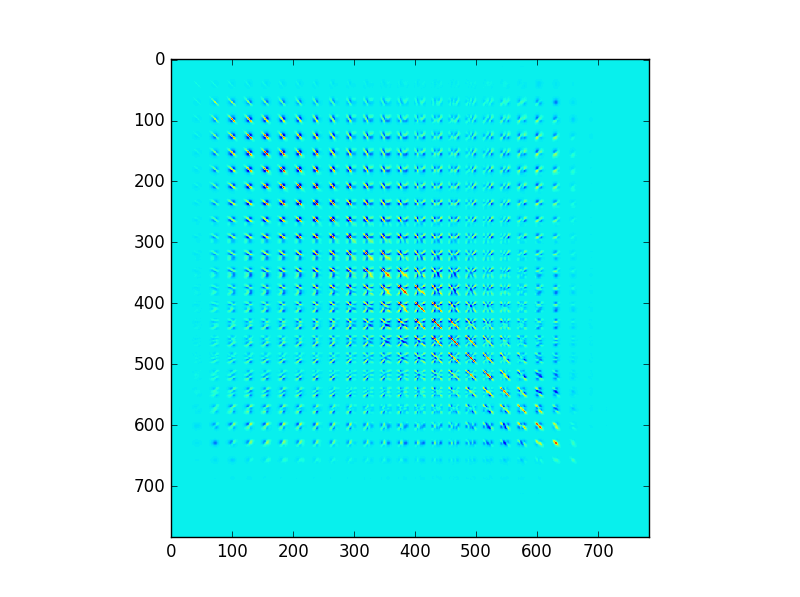
\includegraphics[scale=.75]{images/covariance_for_6.png}
    Above is the visualization for the covariance matrix of 6. Terms close to the diagonal tend to have a higher covariance than terms further away from the diagonals. This indicates that adjacent pixels are have more importance than pixels far away from each other.
    \end{mdframed}
    
    \item Classify the digits in the test set on the basis of posterior probabilities with two different approaches.
    \begin{enumerate}[label=(\roman*)]
        \item Linear discriminant analysis (LDA). Model the class conditional probabilities as Gaussians $\N(\mu_C, \Sigma)$ with different means $\mu_C$ (for class C) and the same covariance matrix $\Sigma$, the average covariance matrix of the 10 classes. \\
        
        Hold out 10,000 randomly chosen training points for a validation set. Classify each image in the validation set into one of the 10 classes (with a 0-1 loss function). Compute the error rate and plot it over the following numbers of randomly chosen training points: $$[100, 200, 500, 1,000, 2,000, 5,000, 10,000, 30,000, 50,000].$$ (Expect some variance in your error rate when few training points are used.)
        
        \item Quadratic discriminant analysis (QDA). Model the class conditionals as Gaussians $\N(\mu_C, \Sigma_C)$, where $\Sigma_C$ is the estimated covariance matrix for class C. (If any of these covariance matrices turn out singular, implement the trick you described in Q5.(b). You are welcome to use $k$-fold cross validation to choose the right constant(s) for that trick.) Repeat the same tests and error rate calculations you did for LDA.
\newpage        
        \item  (Written answer.) Which of LDA and QDA performed better? Why?
        \begin{mdframed} \solution\\
        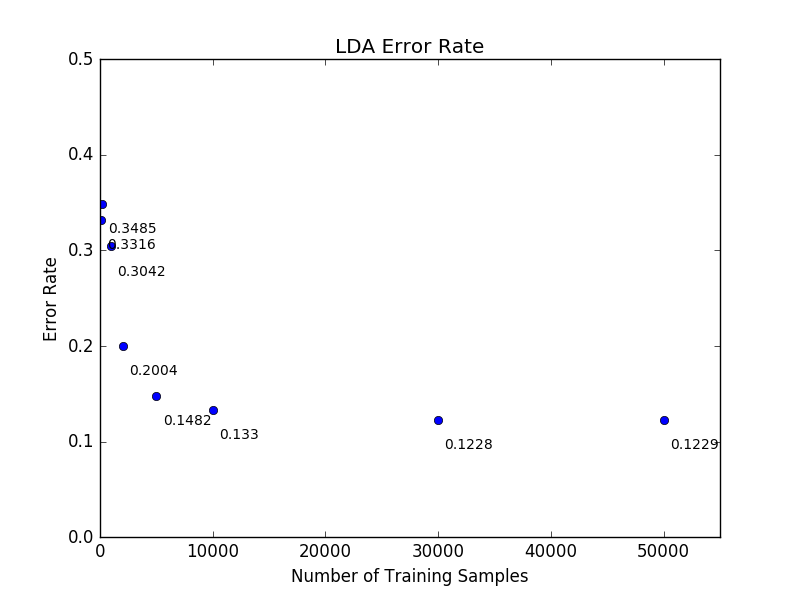
\includegraphics[scale=.5]{images/digit_lda.png}\\
        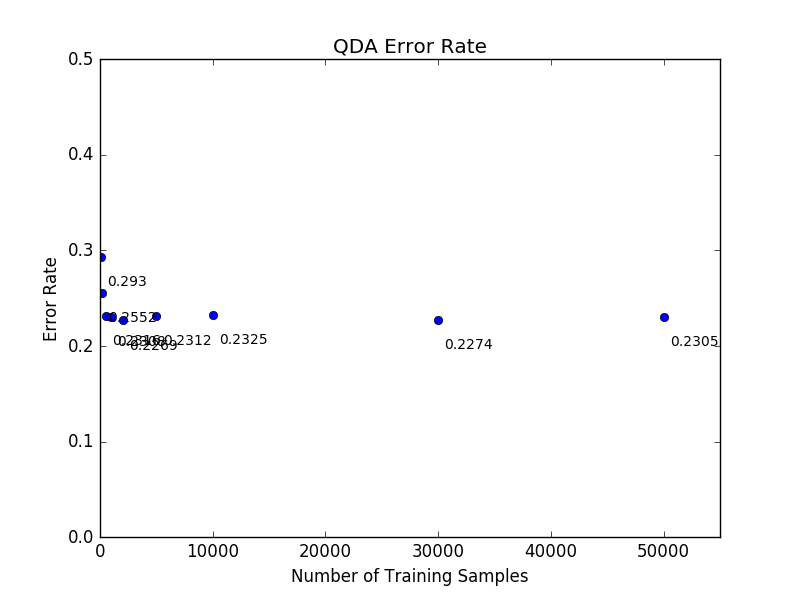
\includegraphics[scale=.5]{images/digit_qda.png}
               
        LDA performed better than QDA. This is because QDA is prone to overfitting, especially when there aren't enough samples.
        
        \end{mdframed}
        
        \item Train your best classifier with \texttt{train.mat} and classify the images in \texttt{test.mat}. Submit your labels to the online Kaggle competition. Record your optimum prediction rate in your submission. You are welcome to compute extra features for the Kaggle competition. If you do so, please describe your implementation in your assignment. Please use extra features \textbf{only} for this portion of the assignment. In your submission, include plots of error rate versus number of training examples for both LDA and QDA. Also include tables giving the error rates (as percentages) for each number of training examples for both LDA and QDA. Include written answers where indicated.
        \begin{mdframed} \solution
        I used the entire training set to train an LDA classifier. I didn't use any extra features. My best accuracy for the kaggle submission was 0.88360.
        \begin{center}
        LDA Table:
        \begin{tabular}{|c c|}
        \hline
        Samples & Error Rate\\
        \hline
        100 & 0.3316\\
        200 & 0.3485\\
        500 & 0.6763\\
        1000 & 0.3042\\
        2000 & 0.2004\\
        5000 & 0.1482\\
        10000 & 0.1330\\
        30000 & 0.1228\\
        50000 & 0.1229\\
        \hline
        \end{tabular}
        \quad QDA Table:
        \begin{tabular}{|c c|}
        \hline
        Samples & Error Rate\\
        \hline
        100 & 0.2930\\
        200 & 0.2552\\
        500 & 0.2316\\
        1000 & 0.2308\\
        2000 & 0.2269\\
        5000 & 0.2312\\
        10000 & 0.2325\\
        30000 & 0.2274\\
        50000 & 0.2305\\
        \hline
        \end{tabular}
        \end{center}
        \end{mdframed}
    
    \end{enumerate}
    \item Next, apply LDA or QDA (your choice) to spam. Submit your test results to the online Kaggle competition. Record your optimum prediction rate in your submission. If you use additional features (or omit features), please describe them. \\
    
    \emph{Optional:} If you use the defaults, expect relatively low classification rates. The TAs suggest using a bag-of-words model. You may use third-party packages to implement that if you wish. Also, normalizing your vectors might help.
    
    \begin{mdframed} \solution
    I used LDA and used a bag of words model with a hash to 2048 buckets for each feature word. This got me an accuracy of 0.92960.
    \end{mdframed}
\end{enumerate}

\newpage
\section*{Appendix}
The following code was used to generate iscontour graphs:
\begin{python}
import matplotlib
import numpy as np
import matplotlib.cm as cm
import matplotlib.mlab as mlab
import matplotlib.pyplot as plt

matplotlib.rcParams['xtick.direction'] = 'out'
matplotlib.rcParams['ytick.direction'] = 'out'

def graph(part, m1, m2, x_min, x_max, y_min, y_max, delta=.025):
    x = np.arange(x_min, x_max, delta)
    y = np.arange(y_min, y_max, delta)
    X, Y = np.meshgrid(x, y)
    mux, muy, sigmax, sigmay, sigmaxy = m1
    Z1 = mlab.bivariate_normal(X, Y, sigmax, sigmay, mux, muy, sigmaxy)
    if m2:
        mux, muy, sigmax, sigmay, sigmaxy = m2
        Z2 = mlab.bivariate_normal(X, Y, sigmax, sigmay, mux, muy, sigmaxy)
        Z = Z1 - Z2
    else:
        Z = Z1
    plt.figure()
    CS = plt.contour(X, Y, Z)
    plt.clabel(CS, inline=1, fontsize=10)
    plt.title('Isocontour for part (' + part + ')')

def part_a():
    m1 = [1, 1, 1, 2**.5, 0]
    m2 = None
    x_min, x_max = -4, 4
    y_min, y_max = -4, 4
    graph('a', m1, m2, x_min, x_max, y_min, y_max)

def part_b():
    m1 = [-1, 2, 2**.5, 3**.5, 1]
    m2 = None
    x_min, x_max = -4, 4
    y_min, y_max = -4, 4
    graph('b', m1, m2, x_min, x_max, y_min, y_max)

def part_c():
    m1 = [0, 2, 2**.5, 1, 1]
    m2 = [2, 0, 2**.5, 1, 1]
    x_min, x_max = -4, 4
    y_min, y_max = -4, 4
    graph('c', m1, m2, x_min, x_max, y_min, y_max)

def part_d():
    m1 = [0, 2, 2**.5, 1, 1]
    m2 = [2, 0, 2**.5, 3**.5, 1]
    x_min, x_max = -4, 4
    y_min, y_max = -4, 4
    graph('d', m1, m2, x_min, x_max, y_min, y_max)

def part_e():
    m1 = [1, 1, 2**.5, 1, 0]
    m2 = [-1, -1, 2**.5, 2**.5, 1]
    x_min, x_max = -4, 4
    y_min, y_max = -4, 4
    graph('e', m1, m2, x_min, x_max, y_min, y_max)

part_a()
part_b()
part_c()
part_d()
part_e()

plt.show()
\end{python}
\newpage

The following code was used to generate and do calculations on the random samples in question 3:
\begin{python}
import matplotlib
import numpy as np
import matplotlib.cm as cm
import matplotlib.mlab as mlab
import matplotlib.pyplot as plt

matplotlib.rcParams['xtick.direction'] = 'out'
matplotlib.rcParams['ytick.direction'] = 'out'

X1 = np.random.normal(3, 3, 100)
X2 = np.random.normal(.5*X1 + 4, 2)

x1_mean, x2_mean = np.mean(X1), np.mean(X2)

Sigma = np.cov(X1, X2)

eig_vals, eig_vectors = np.linalg.eig(Sigma)

v1, v2 = eig_vectors[:,0], eig_vectors[:,1]

v1, v2 = v1 / np.linalg.norm(v1), v2 / np.linalg.norm(v2)

v1_x = v1[0] * eig_vals[0]
v1_y = v1[1] * eig_vals[0]

v2_x = v2[0] * eig_vals[1]
v2_y = v2[1] * eig_vals[1]

string = "Randomly generated (X1, X2) coordinate pairs:\n"
for i in range(100):
    x1, x2 = X1[i], X2[i]
    s = '(' + str(x1) + ', ' + str(x2) + ')\n'
    string += s

string += '\n\n' + str('Mean of the sample: (' + str(x1_mean) + ', ' + str(x2_mean) + ')\n\n')
string += '2x2 Covariance Matrix:\n'
string += '[ ' + str(Sigma[0][0]) + '  ' + str(Sigma[0][1]) + ' ]\n'
string += '[ ' + str(Sigma[1][0]) + '  ' + str(Sigma[1][1]) + ' ]\n\n'
string += 'Eigenvalues and Eigenvectors of the Covariance Matrix:\n'
string += 'v1: ' + str(v1) + '  lambda1: ' + str(eig_vals[0]) + '\n'
string += 'v2: ' + str(v2) + '  lambda2: ' + str(eig_vals[1]) + '\n'

f = open('question_3.txt', 'w', encoding='utf-8')
f.write(string)
f.close()

plt.figure(figsize=(7.5, 7.5))
plt.xlabel("X1")
plt.ylabel("X2")
plt.axis((-15, 15, -15, 15))
plt.plot(X1, X2, 'ro')
plt.arrow(x1_mean, x2_mean, v1_x, v1_y, length_includes_head=True, head_width=.5, color='blue')
plt.arrow(x1_mean, x2_mean, v2_x, v2_y, length_includes_head=True, head_width=.5, color='blue')

ut = np.array([v1, v2])
x_rotated = np.dot(ut, np.array([X1 - x1_mean, X2 - x2_mean]))
plt.figure(figsize=(7.5, 7.5))
plt.axis((-15, 15, -15, 15))
plt.plot(x_rotated[0], x_rotated[1], 'mo')
plt.arrow(0, 0, eig_vals[0], 0, length_includes_head=True, head_width=.5, color='cyan')
plt.arrow(0, 0, 0, eig_vals[1], length_includes_head=True, head_width=.5, color='cyan')

plt.show()
\end{python}
\newpage

The following code was used for MNIST:
\begin{python}
import numpy as np
import scipy.io
import matplotlib.pyplot as plt
import csv
import sys

traindatafilename = "hw3_mnist_dist/train"
traindata = scipy.io.loadmat(traindatafilename)
traindata = traindata['trainX']

VAL_SIZE = 10000

def normalize(sample):
    return sample / np.linalg.norm(sample)

def visualize_covariance_matrix(digit):
    digit_data = []
    for sample in traindata:
        if sample[-1] == digit:
            digit_data.append(normalize(sample[:-1]))
    sigma = np.cov(np.transpose(digit_data))
    plt.imshow(sigma, interpolation='nearest')
    #plt.colorbar()
    plt.show()

def average_covariance_matrix(samples, labels):
    covs = []
    for i in range(10):
        sig_i = covariance_matrix_for_digit(i, samples, labels)
        covs.append(sig_i)
    a = np.mean(covs, axis=0)
    return np.mean(covs, axis=0)

def covariance_matrix_for_digit(digit, samples, labels):
    digit_samples = []
    for i in range(len(labels)):
        if labels[i] == digit:
            sample = samples[i]
            digit_samples.append(normalize(sample))
    sigma = np.cov(np.transpose(digit_samples))
    return sigma

def mean_for_digit(digit, samples, labels):
    digit_samples = []
    for i in range(len(labels)):
        if labels[i] == digit:
            sample = samples[i]
            digit_samples.append(normalize(sample))
    return np.mean(np.transpose(digit_samples), axis=1)

np.random.shuffle(traindata)
validation = traindata[:VAL_SIZE]
training = traindata[VAL_SIZE:]

training_samples = training[:,:-1]
temp = training[:,784:]
training_labels = temp.reshape(temp.shape[0])

validation_samples = validation[:,:-1]
temp = validation[:,784:]
validation_labels = temp.reshape(temp.shape[0])

def plot_lda():
    num_points = [100, 200, 500, 1000, 2000, 5000, 10000, 30000, 50000]
    accuracy_list = []
    for N in num_points:
        print(N)
        sys.stdout.flush()
        temp_samples = training_samples[:N]
        temp_labels = training_labels[:N]
        covariance = average_covariance_matrix(temp_samples, temp_labels)
        if np.linalg.det(covariance) == 0:
            covariance += (10**-10)*np.eye(784)
        precision = np.linalg.inv(covariance)
        mu_c = [mean_for_digit(i, temp_samples, temp_labels) for i in range(10)]
        mu_dot_precision = [np.dot(np.transpose(mu_c[i]), precision) for i in range(10)]
        wrong = 0
        for i in range(VAL_SIZE):
            sample = validation_samples[i]
            sample = normalize(sample)
            max_val = float('-inf')
            classification = -1
            for c in range(10):
                val = np.dot(mu_dot_precision[c], sample)
                val -= .5*np.dot(mu_dot_precision[c], mu_c[c])
                if val > max_val:
                    max_val = val
                    classification = c
            if classification != validation_labels[i]:
                wrong += 1
        accuracy_list.append(wrong / VAL_SIZE)
    plt.plot(num_points, accuracy_list, 'bo')
    plt.axis([0, 55000, 0, 1])
    plt.title("LDA Error Rate")
    plt.ylabel("Error Rate")
    plt.xlabel("Number of Training Samples")
    for i in range(len(accuracy_list)):
        text = str(accuracy_list[i])
        x = num_points[i]
        y = accuracy_list[i]
        plt.annotate(text, xy = (x, y), xytext = (x + 560, y - .03), fontsize = 10)
    print(accuracy_list)
    sys.stdout.flush()
    plt.show()

def plot_qda():
    num_points = [100, 200, 500, 1000, 2000, 5000, 10000, 30000, 50000]
    accuracy_list = []
    for N in num_points:
        print(N)
        sys.stdout.flush()
        temp_samples = training_samples[:N]
        temp_labels = training_labels[:N]
        covariance_c = []
        for i in range(10):
            cov = covariance_matrix_for_digit(i, temp_samples, temp_labels)
            if np.linalg.det(cov) == 0:
                cov += (1)*np.eye(784)
            covariance_c.append(cov)
        precision_c = [np.linalg.inv(cov) for cov in covariance_c]
        log_det_c = [np.log(np.linalg.det(cov)) for cov in covariance_c]
        mu_c = [mean_for_digit(i, temp_samples, temp_labels) for i in range(10)]
        #mu_dot_precision = [np.dot(np.transpose(mu_c[i]), precision_c[i]) for i in range(10)]
        wrong = 0
        for i in range(VAL_SIZE):
            sample = validation_samples[i]
            sample = normalize(sample)
            max_val = float('-inf')
            classification = -1
            for c in range(10):
                y = sample - mu_c[c]
                val = -np.dot(np.dot(np.transpose(y), precision_c[c]), y)
                val -= log_det_c[c]
                if val > max_val:
                    max_val = val
                    classification = c
            if classification != validation_labels[i]:
                wrong += 1
        accuracy_list.append(wrong / VAL_SIZE)
    plt.plot(num_points, accuracy_list, 'bo')
    plt.axis([0, 55000, 0, 1])
    plt.title("QDA Error Rate")
    plt.ylabel("Error Rate")
    plt.xlabel("Number of Training Samples")
    for i in range(len(accuracy_list)):
        text = str(accuracy_list[i])
        x = num_points[i]
        y = accuracy_list[i]
        plt.annotate(text, xy = (x, y), xytext = (x + 560, y - .03), fontsize = 10)
    print(accuracy_list)
    sys.stdout.flush()
    plt.show()

def predict_test_set():
    all_samples = traindata[:,:-1]
    temp = traindata[:,784:]
    all_labels = temp.reshape(temp.shape[0])
    covariance = average_covariance_matrix(all_samples, all_labels)
    if np.linalg.det(covariance) == 0:
        covariance += (10**-10)*np.eye(784)
    precision = np.linalg.inv(covariance)
    mu_c = [mean_for_digit(i, all_samples, all_labels) for i in range(10)]
    mu_dot_precision = [np.dot(np.transpose(mu_c[i]), precision) for i in range(10)]
    guesses = []
    testdatafilename = "hw3_mnist_dist/test"
    testdata = scipy.io.loadmat(testdatafilename)
    testdata = testdata['testX']
    for sample in testdata:
        x = normalize(sample)
        max_val = float('-inf')
        classification = -1
        for c in range(10):
            val = np.dot(mu_dot_precision[c], x)
            val -= .5*np.dot(mu_dot_precision[c], mu_c[c])
            if val > max_val:
                max_val = val
                classification = c
        guesses.append(classification)

    with open('mnist_submission_1.csv', 'w', newline='') as csvfile:
        writer = csv.writer(csvfile)
        writer.writerow(['Id', 'Category'])
        i = 0
        for g in guesses:
            writer.writerow([i, g])
            i += 1

#visualize_covariance_matrix(6)
#plot_lda()
#plot_qda()
#predict_test_set()
\end{python}
\newpage
The following code was used to create the feature vectors for email:
\begin{python}
'''
**************** PLEASE READ ***************

Script that reads in spam and ham messages and converts each training example
into a feature vector

Code intended for UC Berkeley course CS 189/289A: Machine Learning

Requirements:
-scipy ('pip install scipy')

To add your own features, create a function that takes in the raw text and
word frequency dictionary and outputs a int or float. Then add your feature
in the function 'def generate_feature_vector'

The output of your file will be a .mat file. The data will be accessible using
the following keys:
    -'training_data'
    -'training_labels'
    -'test_data'

'''

from collections import defaultdict
import glob
import re
import scipy.io

NUM_TEST_EXAMPLES = 10000
NUM_FEATURES = 2048

BASE_DIR = './'
SPAM_DIR = 'spam/'
HAM_DIR = 'ham/'
TEST_DIR = 'test/'

# ************* Features *************

# Generates a feature vector
def generate_feature_vector(text, freq):
    feature = [0 for i in range(NUM_FEATURES)]
    for word in freq:
        feature[hash(word)] += freq[word]
    return feature

# This method generates a design matrix with a list of filenames
# Each file is a single training example

def hash(word):
    num = 0
    for letter in word:
        num = (num + ord(letter)) % NUM_FEATURES
        num = (num * 31) % NUM_FEATURES
    return num

def generate_design_matrix(filenames):
    global word_to_index, count
    design_matrix = []
    for filename in filenames:
        with open(filename) as f:
            text = f.read() # Read in text from file
            text = text.replace('\r\n', ' ') # Remove newline character
            words = re.findall(r'\w+', text)
            word_freq = defaultdict(int) # Frequency of all words
            for word in words:
                word_freq[word] += 1

            # Create a feature vector
            feature_vector = generate_feature_vector(text, word_freq)
            design_matrix.append(feature_vector)
    return design_matrix

# ************** Script starts here **************
# DO NOT MODIFY ANYTHING BELOW

# Important: the test_filenames must be in numerical order as that is the
# order we will be evaluating your classifier

spam_filenames = glob.glob(BASE_DIR + SPAM_DIR + '*.txt')
spam_design_matrix = generate_design_matrix(spam_filenames)
ham_filenames = glob.glob(BASE_DIR + HAM_DIR + '*.txt')
ham_design_matrix = generate_design_matrix(ham_filenames)
test_filenames = [BASE_DIR + TEST_DIR + str(x) + '.txt' for x in range(NUM_TEST_EXAMPLES)]
test_design_matrix = generate_design_matrix(test_filenames)

X = spam_design_matrix + ham_design_matrix
Y = [1]*len(spam_design_matrix) + [0]*len(ham_design_matrix)

file_dict = {}
file_dict['training_data'] = X
file_dict['training_labels'] = Y
file_dict['test_data'] = test_design_matrix
scipy.io.savemat('spam_data.mat', file_dict, do_compression=True)
\end{python}
\newpage
The following code was used to classify emails:
\begin{python}
import numpy as np
import scipy.io
import matplotlib.pyplot as plt
import csv

traindatafilename = "dist/spam_data"
data = scipy.io.loadmat(traindatafilename)

traindata = data['training_data']
NUM_FEATURES = traindata.shape[1]
testdata = data['test_data']
labels = data['training_labels']
labels = labels.transpose()
traindata = np.append(traindata, labels, axis=1)
np.random.shuffle(traindata)

SIZE = traindata.shape[0]

def average_covariance_matrix(samples, labels):
    covs = []
    for i in range(2):
        sig_i = covariance_matrix_for_digit(i, samples, labels)
        covs.append(sig_i)
    a = np.mean(covs, axis=0)
    return np.mean(covs, axis=0)

def covariance_matrix_for_digit(digit, samples, labels):
    digit_samples = []
    for i in range(len(labels)):
        if labels[i] == digit:
            sample = samples[i]
            digit_samples.append(sample)
    sigma = np.cov(np.transpose(digit_samples))
    return sigma

def mean_for_digit(digit, samples, labels):
    digit_samples = []
    for i in range(len(labels)):
        if labels[i] == digit:
            sample = samples[i]
            digit_samples.append(sample)
    return np.mean(np.transpose(digit_samples), axis=1)

def predict_test_set():
    all_samples = traindata[:,:-1]
    temp = traindata[:,-1]
    all_labels = temp.reshape(temp.shape[0])
    covariance = average_covariance_matrix(all_samples, all_labels)
    if np.linalg.det(covariance) == 0:
        covariance += (10**-10)*np.eye(covariance.shape[0])
    precision = np.linalg.inv(covariance)
    mu_c = [mean_for_digit(i, all_samples, all_labels) for i in range(2)]
    mu_dot_precision = [np.dot(np.transpose(mu_c[i]), precision) for i in range(2)]
    guesses = []
    testdata = data['test_data']
    for sample in testdata:
        max_val = float('-inf')
        classification = -1
        for c in range(2):
            val = np.dot(mu_dot_precision[c], sample)
            val -= .5*np.dot(mu_dot_precision[c], mu_c[c])
            if val > max_val:
                max_val = val
                classification = c
        guesses.append(classification)

    with open('email_submission_2.csv', 'w', newline='') as csvfile:
        writer = csv.writer(csvfile)
        writer.writerow(['Id', 'Category'])
        i = 0
        for g in guesses:
            writer.writerow([i, g])
            i += 1

predict_test_set()
\end{python}
\newpage
The following is the output generated for question 3:
Randomly generated (X1, X2) coordinate pairs:
(3.7521175467, 8.16282191925)
(3.73391265331, 3.73692789908)
(2.70265892424, 4.26963073306)
(4.86408111135, 4.68777535408)
(4.04996547861, 8.52137345053)
(0.233585312481, 2.15123211979)
(4.6041917731, 7.2489443482)
(7.61034713427, 10.9542777426)
(4.72002603227, 5.12168028497)
(5.41094430384, 5.16519508061)
(0.459242421478, 8.11592405812)
(1.78226363989, 7.06870992236)
(2.116677488, 3.80815299087)
(4.28912284523, 3.73386111723)
(-1.20508177032, 3.05643076294)
(3.59804401979, 4.11822629615)
(5.51393190387, 6.86667784866)
(8.36242717957, 9.53571465398)
(5.4260122171, 5.91928259072)
(2.7537091697, 4.93237819492)
(2.04891141963, 7.32403449486)
(0.748471184937, 4.62601087149)
(4.15245649992, 5.94312110212)
(1.78357721872, 6.26133256458)
(10.0761489622, 6.77027228948)
(0.138413300709, 2.53665664087)
(6.99021469216, 6.1641337023)
(4.87779171263, 5.39949550732)
(2.18027215697, 3.58818823937)
(4.37601828977, 7.37743391943)
(-0.403906529854, 5.81261300152)
(7.238750534, 10.6662821816)
(5.28203164971, 2.94781817055)
(1.47698398904, 8.20416053038)
(7.20651817719, 9.41422367258)
(3.49733793096, 6.45590328222)
(-1.69876384519, 5.79097651739)
(2.27003188283, 3.37284905493)
(5.30524529387, 7.11735793531)
(-0.708743055773, 0.482898466813)
(4.2870282026, 4.44456096796)
(1.72207660836, 5.89640056627)
(-1.6517916951, 4.71782119047)
(3.64688496845, 3.66853483026)
(-2.2827375063, 5.97301417881)
(7.25073767216, 6.37548725623)
(0.0219264150681, 6.96496629942)
(2.74697859131, 6.87842980029)
(0.9756375313, 4.84214203557)
(4.76849265075, 6.66296858189)
(2.16081243452, 5.45820445858)
(1.24863153362, 2.99793038347)
(4.75858704212, 9.8135639022)
(4.89645001619, 7.34263981384)
(6.42608031055, 7.02770794576)
(-1.02759017108, 2.09117174852)
(3.66932901205, 4.41362239498)
(-1.08946594404, 7.15087615645)
(-1.76798897241, 7.52923836434)
(0.995156340805, 4.60838990299)
(4.42938055378, 5.96424552889)
(2.8934711714, 5.22153654127)
(-0.596211986939, 2.72329479959)
(-1.46150025031, 4.4853773386)
(-1.16934708588, 2.26598335086)
(5.59908657819, 5.52978970593)
(5.70448750525, 7.38130788361)
(-0.0187030345345, 3.90452664791)
(-1.1393847661, 4.36508787994)
(0.569516503028, 3.73446717284)
(5.47268425414, 8.26298109484)
(2.6891642399, 5.51421415364)
(1.08901866141, 2.37888154817)
(3.18606821271, 4.88315663582)
(3.64956226008, 7.85649646802)
(-3.81778994737, 0.420001763923)
(3.20750224283, 2.96644376565)
(-0.60486149933, 3.8036331458)
(2.05047250718, 7.48677710128)
(5.10477389266, 6.04332776735)
(1.54512778571, 4.82244209302)
(9.051931535, 7.96438147131)
(3.10644302141, 9.89500236358)
(4.04500482586, 6.99686365435)
(5.82984625996, 5.20447418659)
(5.07670223739, 5.22255409667)
(0.977815451684, 3.96130215949)
(2.56488355916, 7.50649118358)
(-3.11286944807, 2.40380193893)
(1.76053573535, 3.57379389433)
(2.35464075444, 5.87572003681)
(4.16260353484, 5.8968119939)
(8.84843453206, 8.97763053233)
(4.28992162475, 4.03992119306)
(3.06456772803, 7.01061363361)
(2.04998482517, 8.03397479395)
(5.25272084205, 3.91833857725)
(2.37940197049, 6.64065930299)
(-0.0119824838814, 4.41464457074)
(8.53727739727, 8.21954678402)


Mean of the sample: (2.91981557591, 5.64059149046)

2x2 Covariance Matrix:
[ 8.31478388898  3.34988838329 ]
[ 3.34988838329  4.61656028265 ]

Eigenvalues and Eigenvectors of the Covariance Matrix:
v1: [ 0.8611786   0.50830249]  lambda1: 10.2920236955
v2: [-0.50830249  0.8611786 ]  lambda2: 2.63932047611



\end{document}
